\chapter[Studium przypadku: Dynamicznie generowany panel administracyjny]{Studium przypadku: Dynamicznie generowany panel administracyjny}
  \section{Wstęp}
  Świat technologii informatycznych zmienia się bardzo szybko. Ogromnemu skokowi mocy obliczeniowej sprzętu komputerowego towarzyszył w ostatnich kilku latach znaczący spadek cen związanych z jego wykorzystaniem. Stało się to katalizatorem rozwoju nowych trendów między innymi w dziedzinie wytwarzania oprogramowania. Gwałtowny wzrost zainteresowania dynamicznymi językami programowania takimi jak Ruby, Python czy JavaScript oraz pojawienie się nowych metodyk rozwoju produktów informatycznych, które coraz częściej ujmują ten proces bardziej z filozoficznego aniżeli technicznego lub biznesowego punktu widzenia jest bez wątpienia jednym z owoców tego procesu.
  
  Spadek kosztów mocy obliczeniowej skutecznie rozwiązał problem wyboru technologii realizacji projektu informatycznego: wydajność narzędzi, których użyjemy do realizacji celu stała się w większości przypadków pomijalnym lub przynajmniej drugorzędnym problemem. Dziś najważniejszym kryterium wyboru jest stopień dopasowania możliwości oraz charakterystyki rozważanej technologii do potrzeb zespołu odpowiedzialnego za rozwój projektu. Oczywiście istnieją również skrajne przypadki, w których to oprogramowanie, z różnych przyczyn, musi zostać napisane w konkretnej technologii. Te smutne przypadki stanowią jednak kroplę w morzu wykraczającą daleko poza ramy niniejszej pracy.
  
  W czasach, kiedy o wiele bardziej opłaca się dokupić nowy serwer niż pokrywać koszty optymalizacji ogromną furorę robi termin \"Przedwczesna optymalizacja\". Te dwa słowa mają dzisiaj znaczenie negatywne, które jest jednak jak najbardziej uzasadnione z ekonomicznego oraz użytkowego punktu widzenia. Dopóki niedostatki w wydajności oprogramowania można skompensować inwestycją w nowe zasoby sprzętowe zespół programistów powinien skupiać wszystkie swoje wysiłki na rozwój funkcjonalności. Optymalizacja kodu następuje dopiero w momencie, kiedy koszty inwestycji w sprzęt przewyższają koszt związane z optymalizacją albo w momencie kiedy oprogramowanie ze względu na swoją nie optymalność przestaje się skalować na nowe zasoby sprzętowe.
  
  Na pierwszy rzut oka może wydawać się, że ten wstęp niewiele ma wspólnego z tematem pracy. Należy jednak uświadomić sobie, że to właśnie opisane powyżej zmiany w sposobie myślenia o metodach prowadzenia projektów IT stoją u podstaw rozwoju nowoczesnych narzędzi takich jak wymienione wcześniej dynamiczne języki, wysokopoziomowe frameworki programistyczne na nich oparte czy metodologie pokroju Behaviour Driven Development. Środki, które służą osiągnięciu założonego celu są jedną z najważniejszych zmiennych od których zależy sukces projektu, w przeszłości istniało wiele barier ograniczających ich wybór, dziś większość z nich została usunięta.
  
  \section{Założenia projektu}
  Celem niniejszego rozdziału jest pokazanie czytelnikowi w jaki sposób rozwija się konkretny projekt prowadzony w zgodzie z metodologią BDD oraz jakie płyną z tego korzyści. Wybrany temat projektu to dynamiczny panel administracyjny dla aplikacji internetowych opartych na bibliotece Ruby on Rails, jego główne założenia to:
  
  \begin{description}
    \item[Uniwersalność] Panel powinien współpracować z większością aplikacji napisanych w Ruby on Rails. W praktyce oznacza to, że jeśli modele biznesowe powinny być klasami pochodnymi klasy \verb+ActiveRecord+ a sposób budowy aplikacji jest zgodny z konwencjami przyjętymi dla aplikacji Ruby on Rails.
    \item[CRUD] W teorii baz danych istnieją cztery podstawowe operacje jakie możemy wykonać na zasobie: Tworzenie, odczytanie, aktualizacja, usunięcie (ang. Create, read, update and delete). Biblioteka ma pozwalać na zarządzanie modelami biznesowymi aplikacji przy użyciu jedynie tych czterech standardowych metod.
    \item[Dynamiczność] Po instalacji panel powinien sam wykryć rodzaje zasobów na jakich operuje aplikacja oraz wygenerować odpowiednie widoki i formularze do zarządzania nimi. Zmiany w budowie modeli biznesowych, które wymuszają konieczność zmian w zarządzaniu nimi, jak również pojawienie się nowych modeli również powinno być odzwierciedlone w zachowaniu panelu automatycznie, bez konieczności jakiejkolwiek ingerencji.
    \item[Proste wdrożenie] Podstawowe wdrożenie rozwiązania wymaga jedynie aby aplikacja kliencka korzystała z biblioteki Ruby on Rails w wersji co najmniej 3.0.3. Po dodaniu biblioteki panelu do listy gemów wykorzystywanych przez aplikację możliwe jest natychmiastowe korzystanie.
    \item[Wygoda użytkowania] Proces zarządzania aplikacją powinien być jak najwygodniejszy. Oznacza to między innymi, że pola formularzy służących do tworzenia lub edycji rekordów powinny być dostosowane do rodzaju danych jakie przechowują a próby wprowadzenia nieprawidłowych wartości powinny być sygnalizowane czytelną informacją o błędzie. Jeśli istnieją powiązania pomiędzy kilkoma modelami biznesowymi, to powinna istnieć bardzo szybka możliwość zarządzania każdym z powiązanych rekordów.
  \end{description}
  
  \subsection{Open Source}
    Biblioteka jest dostępna za darmo na zasadach licencji MIT.\footnote{http://en.wikipedia.org/wiki/MIT\_License} Filozofia rozwoju oprogramowania na zasadach open source jest bardzo bliska środowisku programistów Ruby. Sam język udostępniony jest na licencji GPL, biblioteka Ruby on Rails korzysta z licencji MIT. Użycie licencji MIT oznacza, że każdy otrzymuje prawo do nielimitowanego wykorzystania kopii oprogramowania w dowolny sposób, sprawia to, że jest to najchętniej wykorzystywana przez programistów Ruby licencja.
    
  \subsection{Sposób prowadzenia projektu}
  Projekt prowadzony jest według bardzo uproszczonych zasad metodologii SCRUM.\footnote{http://en.wikipedia.org/wiki/Scrum\_(development)} Rozwój projektu podzielony jest na tygodniowe sprinty, przed każdym z nich następuje spotkanie zespołu, podczas którego wybierane i przydzielane są konkretne zadania do wykonania w następnej iteracji. Spotkania te służą również omówieniu bieżących spraw związanych z projektem.
  
  Zespół zaangażowany w projekt składa się z trzech osób: dwóch programistów, oraz osoby dzielącej rolę Scrum Mastera, który odpowiedzialny jest za przygotowanie i prowadzenie spotkań oraz Product Ownera, który reprezentuje oczekiwania końcowego użytkownika dotyczące kwestii funkcjonalności oraz ekonomicznych kwestii związanych z rozwojem projektu.
  
  Duży nacisk kładziony jest na testowanie oprogramowania, testy akceptacyjne istnieją w formie zautomatyzowanych scenariuszy BDD. Każda funkcjonalność lub modyfikacja oprogramowania akceptowana jest jedynie jeśli dostarczona jest wraz z pełnym zestawem testów ją dokumentujących.
  
  \subsection{Dodatkowe narzędzia}
  Repozytorium projektu zarządzane jest przez system kontroli wersji GIT\footnote{http://git\-scm.com} a hostowane jest przez serwis GitHub.\footnote{http://github.com} Źródła projektu dostępne są publicznie pod adresem https://github.com/piotrj/administer.
  
  Jako narzędzie wspomagające proces zarządzania projektem użyta została darmowa wersja Pivotal Tracker\footnote{http://www.pivotaltracker.com}, który został zaprojektowany aby wspomagać zarządzanie projektem prowadzonym według zasad SCRUM.
  
  % może inna nazwa?
  \section{Proces implementacji}
  
  Jak zostało to wspomniane wcześniej implementacja podzielona jest na tygodniowe iteracje zwane również sprintami. Każda planowana funkcjonalność zanim zostanie zaimplementowana i stanie się częścią projektu musi zostać krytycznie oceniona pod względem użyteczności oraz opisana w formie krótkiej specyfikacji.
  
  W wypadku kiedy mamy do czynienia z rozbudowaną funkcjonalnością należy podzielić jej implementację na jak najmniejsze, spójne kawałki a każdy z tych fragmentów powinien zostać jasno opisany. Idealnie jest, kiedy fragmenty danej funkcjonalności są od siebie niezależne, to znaczy, jeśli nad każdym z nich można pracować osobno w tym samym czasie. Taka sytuacja niestety zdarza się rzadko. Jeśli dany fragment zależy od innych, należy załączyć taką informację w jego opisie.
  
  Każde nowe zachowanie opisane jest testem w postaci odpowiedniego scenariusza Cucumber. Jest to warunek konieczny, scenariusze powstają przed rozpoczęciem procesu właściwej implementacji, po zaakceptowaniu przez Product Ownera pełnią one rolę testów akceptacyjnych. Testy jednostkowe w postaci specyfikacji RSpec powstają dla części systemu, których szczegóły implementacji są istotne dla prawidłowego jego działania.
  
  \subsection{Aplikacja testowa}
  Specyfika projektu dynamicznego panelu administracyjnego utrudnia nieco pisanie scenariuszy jego użycia. Myśląc o panelu administracyjnym nigdy nie myślimy o nim jako o odrębnym bycie, jest raczej nieodłącznie związany z aplikacją, którą administruje. Aby proces testowania i specyfikowania systemu był jak najbardziej naturalny biblioteka administer rozwijana jest wraz z małą aplikacją testową.
  
  Prosty system blogowy został stworzony, aby opisać i przetestować zachowanie właściwego oprogramowania. Jedynym celem istnienia aplikacji blogowej jest przetestowanie integracji biblioteki administer z zewnętrzną aplikacją. Z technicznego punktu widzenia wszystkie testy behawioralne opisują zachowanie aplikacji testowej, która dołącza bibliotekę administer do puli wykorzystywanych przez siebie gemów. W przypadku oprogramowania, które działa na zasadzie integracji z zewnętrznym systemem taka konfiguracja środowiska testowego jest najlepsza, odpowiada bowiem faktycznemu scenariuszowi użycia. Sam blog jest niezwykle prostą aplikacją, w założeniach ma pozwalać na:
  
  \begin{itemize}
    \item Wyświetlanie artykułów
    \item Tworzenie artykułów
    \item Edycję artykułów
    \item Usuwanie artykułów
    \item Kategoryzację artykułów
    \item Tworzenie kategorii
    \item Edycję kategorii
    \item Usuwanie kategorii
  \end{itemize}
  
  % PRZEREDAGOWAĆ
  Blog świetnie nadaje się do testowania biblioteki typu administer - wszystkie powyższe funkcje, prócz pierwszej, są tak naprawdę funkcjami, które wykonywać ma panel administracyjny. W kontekście tego przykładu cel biblioteki administer jest jasny: Twórca bloga ze swojej strony musi jedynie dołączyć gem administer do projektu, zdefiniować modele biznesowe typu Post czy Kategoria, oraz dopisać akcję odpowiedzialną za wyświetlanie artykułów, cała część odpowiedzialna za akcję zarządzania modelami ma być dynamicznie wykonywana przez gem administer. 
  
  Ilustracja \ref{blog_view} przedstawia stronę z listą artykułów, jest to widok pochodzący z aplikacji testowej. Ilustracja \ref{administer_edit} przedstawia widok edycji rekordu konkretnego artykułu, funkcja ta implementowana jest przez bibliotekę administer.
  
  \begin{figure}[!h]
		\begin{center}
			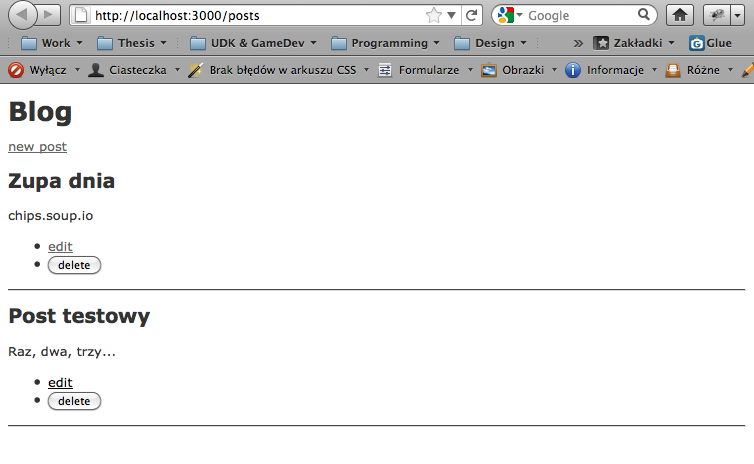
\includegraphics[width=\linewidth]{images/blog.png}
			\caption{Aplikacja testowa - wyświetlanie artykułów}
			\label{blog_view}
		\end{center}
	\end{figure}
	
	\clearpage
	
	\begin{figure}[!h]
		\begin{center}
			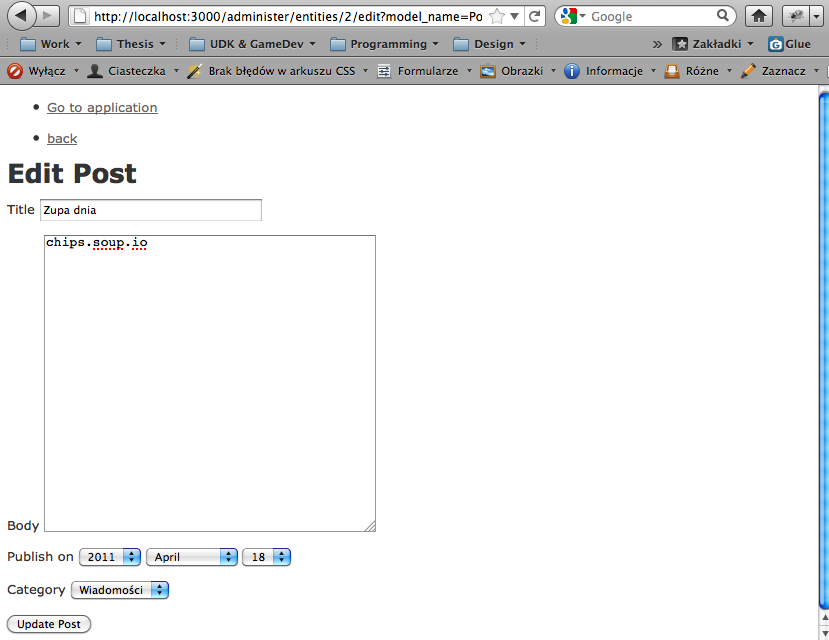
\includegraphics[width=\linewidth]{images/administer_edit.png}
			\caption{administer - edycja rekordu}
			\label{administer_edit}
		\end{center}
	\end{figure}
  
  % lepsza nazwa
  \subsection{Konfiguracja zależności testowych}
    % aplikacja testowa powinna kożystać ze źródeł testowanego gema, nie z jego release
    % Test dependencies - warto coś o tym napisać?
    
  % zdecydowanie zmień nazwę tej sekcji 
  \subsection{Implementacja funkcji usuwania rekordu}
    % screen z listą tiketów
    % dokładny opis całego procesu + wycinki kodu źródłowego dla konkretnego tiketa
    
    Ilustracja \ref{administer_stories}  przedstawia wycinek listy zadań związanych z pracą nad projektem administer a konkretnie są to zadania związane tylko i wyłącznie z rozwojem  panelu administracyjnego.
    
    \clearpage
    
    \begin{figure}
  		\begin{center}
  			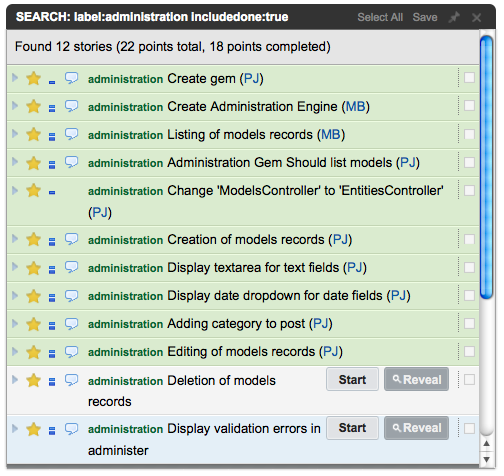
\includegraphics[width=\linewidth]{images/administer_stories_list.png}
  			\caption{Lista zadań do wykonania}
  			\label{administer_stories}
  		\end{center}
  	\end{figure}
  	
    Jako, że projekt jest rozwijany już od jakiegoś czasu, większość zadań z tej listy jest już wykonana, znajdziemy jednak dwa nadal nie rozwiązane problemy:
    
    \begin{itemize}
      \item Deletion of model records
      \item Display validation errors in administer
    \end{itemize}
    
    Skupmy się na rozwiązaniu pierwszego z nich. W momencie pisania tego rozdziału gem administer potrafi już tworzyć, modyfikować oraz wyświetlać informację o rekordach modeli biznesowych aplikacji, która z niego korzysta. Jedną z brakujących funkcji jest usuwanie istniejących rekordów. W tym podrozdziale przeanalizujemy krok po kroku cały cykl wdrażania tej nowej funkcji do istniejącego systemu. Przeanalizowanie tego procesu pomoże nam lepiej zrozumieć sposób w jaki rozwijane jest oprogramowanie w zgodzie z zasadami BDD oraz korzyści z tego płynące.
    
    \subsubsection{Zrozumienie problemu}
    Pierwszy etap pracy to rozpoznanie, z czym tak właściwie mamy do czynienia. Jeśli problem, który mamy rozwiązać został wcześniej udokumentowany, tak jak miało to miejsce w tym wypadku, należy zacząć od dokładnego zaznajomienia się z jego opisem.
    
    Ilustracja \ref{administer_story_desc} przedstawia szczegółowy widok naszego zadania prezentowany przez aplikację Pivotal Tracker, która używana jest jako narzędzie wspomagające proces zarządzania projektem administer.
    
    Podgląd ten informuje nas o wielu rzeczach związanych z zadaniem takich jak status ukończenia, estymacja pracochłonności czy informacja o osobach odpowiedzialnych za zadanie. W kontekście naszych rozważań najważniejszą informacją jaką możemy odczytać z niniejszego podglądu jest jednak opis funkcjonalności. 
    
    Administer rozwijany jest razem z prostą aplikacją testową - systemem blogowym, dlatego wszystkie funkcjonalności opisywane są w kontekście wykorzystania biblioteki przez ten właśnie system. Opis naszego zadania sformułowany jest następująco:
    
    \lstinputlisting{examples/code/ch04/01}
    
    Na pierwszy rzut oka widać, że opis dostarczony został w postaci, której bez modyfikacji można użyć jako scenariusza akceptacyjnego biblioteki cucumber. Należy także zwrócić uwagę na inne ważne cechy tego opisu:
    
    \begin{description}
      \item[Niepodzielność] Dostarczone kroki stanowią minimum, jakie trzeba zaimplementować aby funkcjonalność usuwania rekordów była kompletna.
      \item[Osadzenie w kontekście] Zachowanie zostało opisane w konkretnych warunkach. Mamy informację o stanie początkowym w jakim funkcjonalność powinna działać (Istnieje rekord należący do modelu Post), miejscu oraz zachowaniu które wywoła usunięcie rekordu (Kliknięcie przycisku \verb+Delete+ na stronie z postami) oraz o warunkach końcowych, jakie muszą zostać spełnione w wyniku działania naszej nowej funkcji (Post powinien zniknąć z listy).
    \end{description}
    
    \begin{figure}[h]
  		\begin{center}
  			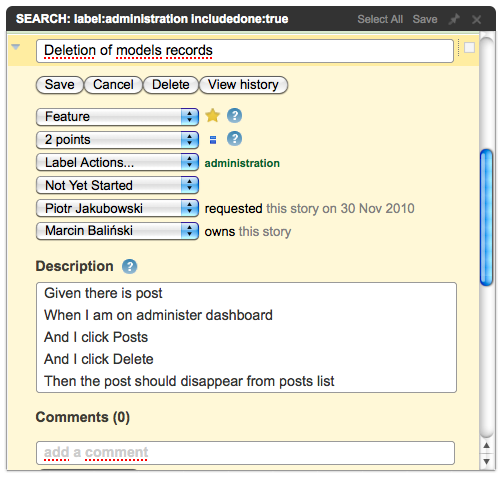
\includegraphics[width=\linewidth]{images/administer_story_desc.png}
  			\caption{Szczegółowy opis zadania}
  			\label{administer_story_desc}
  		\end{center}
  	\end{figure}
  	
  	\subsubsection{Czynności wstępne}
  	
  	Po zapoznaniu się i zrozumieniu istoty problemu, z którym będziemy się zmagać należy przygotować środowisko pracy. W naszym wypadku składają się na to dwie ważne czynności:
  	
  	 \begin{description}
        \item[Upewnienie się, że posiadamy aktualną wersję oprogramowania] Zawsze powinniśmy rozpocząć pracę z najnowszą rozwojową wersją kodu.
        \item[Uruchomienie pełnego zestawu testów] Przed rozpoczęciem pracy należy upewnić się, że wszystkie testy kończą się sukcesem.
      \end{description}
      
    Kod biblioteki administer przechowywany jest w rozproszonym systemie kontroli wersji GIT, spełnienie pierwszego punktu wymaga więc od programisty jedynie synchronizacji swojego lokalnego repozytorium z najnowszą wersją rozwojowej gałęzi kodu znajdującej się w głównym repozytorium. Szczegóły dotyczące operacji na systemie kontroli wersji wykraczają poza ramy tej pracy i zostaną tutaj pominięte. Przyjmijmy jednak, że synchronizacja została wykonana i mamy u siebie najnowszą wersję kodu biblioteki administer. 
    
    Uruchomienie pełnego zestawu testów daje nam pewność, że wersja oprogramowania, na której będziemy pracować spełnia warunki specyfikacji. Nie wolno rozpoczynać pracy jeśli testy z jakiegoś powodu nie przechodzą. W takim wypadku należy najpierw znaleźć przyczynę problemu i zlikwidować go a pracę nad nową funkcjonalnością rozpocząć dopiero kiedy wszystkie testy automatyczne sygnalizują sukces.
    
    Aby uruchomić pełen zestaw testów biblioteki administer wydajemy z głównego katalogu projektu polecenie:
    
    \begin{lstlisting}
      rake
    \end{lstlisting}
    
    Projekt został tak skonfigurowany, że komenda \verb+rake+ wywołana bez dodatkowych parametrów uruchamia zestaw scenariuszy Cucumber oraz testów RSpec opisujących zachowanie biblioteki. 
    
    
    
    \begin{figure}[!h]
  		\begin{center}
  			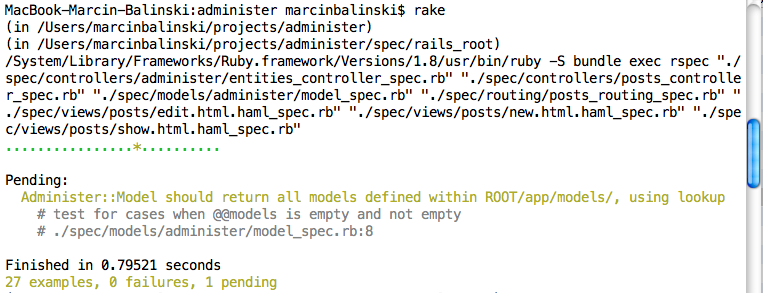
\includegraphics[width=\linewidth]{images/spec_report.png}
  			\caption{Zestaw testów RSpec - raport.}
  			\label{spec_report}
  		\end{center}
  	\end{figure}
  	
  	\clearpage
  	
  	\begin{figure}[!h]
  		\begin{center}
  			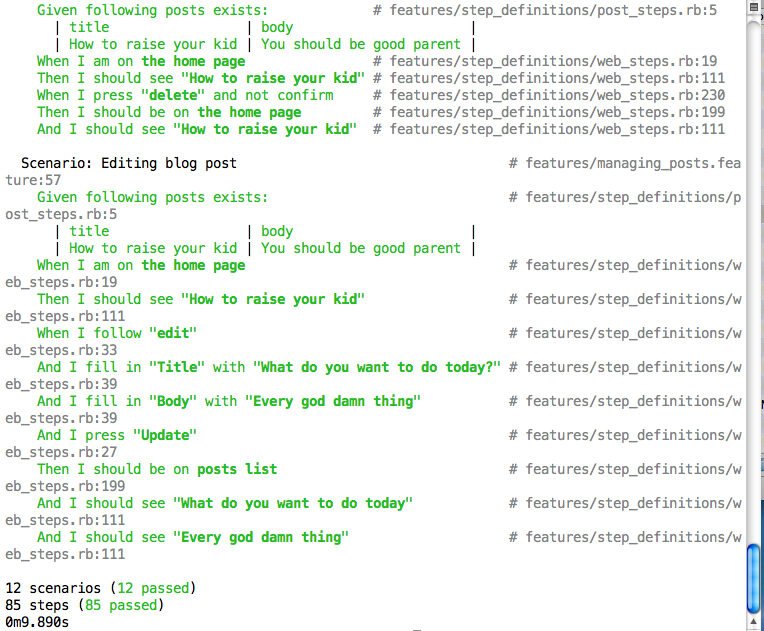
\includegraphics[width=\linewidth]{images/features_report.png}
  			\caption{Zestaw scenariuszy Cucumber - raport.}
  			\label{features_report}
  		\end{center}
  	\end{figure}
  	
  	  Raport po pozytywnym przejściu wszystkich testów powinien wyglądać podobnie jak na ilustracji \ref{spec_report} oraz \ref{features_report}. Oznaczenie \verb+pending+ przy jednym z testów RSpec sygnalizuje, że został tymczasowo wyłączony z zestawu testów przez jednego z programistów. Przyczyny wyłączenia testów mogą być różne, ale proceder ten należy stosować w ostateczności i w pełni świadomie, niedopuszczalne jest wyłączanie testu bez wyraźnego powodu a najlepiej jest, żeby takie sytuacje w ogóle się nie zdarzały.
  	  
  	\subsubsection{Więcej testów}
  	  Proces implementacji zaczyna się od stworzenia scenariusza opisującego nową funkcjonalność. W naszym przypadku scenariusze umieszczone są w podkatalogu \verb+spec/rails_root/features/+. Nas szczególnie interesuje plik \verb+spec/rails_root/features/administer/posts.feature+ w którym opisane jest zachowanie wymagane od panelu administrującego blogiem. W momencie pisania tego rozdziału plik \verb+posts.feature+ wygląda następująco:
  	  
  	\lstinputlisting{examples/code/ch04/02}
  	
  	Powyższe scenariusze opisują zachowanie biblioteki w tym momencie życia projektu, funkcja usuwania rekordu nie jest jeszcze opisana, nie pozostaje nam nic innego jak dopisać odpowiedni scenariusz:
  	
  	\lstinputlisting{examples/code/ch04/03}
  	
  	Oryginalny opis zadania (Ilustracja \ref{administer_story_desc}) został lekko zmodyfikowany w celu lepszego dopasowania do istniejącej infrastruktury i definicji kroków. Powtórne uruchomienie zestawu testów powinno zakończyć się niepowodzeniem - dodany przez nas scenariusz specyfikuje funkcjonalność, której jeszcze nie ma. Sytuację ilustruje zrzut ekranu \ref{scenario_failure}.
  	
  	\clearpage
  	
  	\begin{figure}[!h]
  		\begin{center}
  			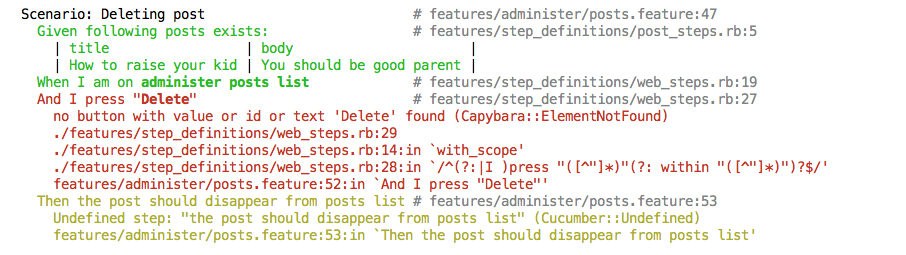
\includegraphics[width=\linewidth]{images/scenario_failure.png}
  			\caption{Nowo dodany scenariusz nie przechodzi}
  			\label{scenario_failure}
  		\end{center}
  	\end{figure}
  	
  	Oprócz informacji o błędzie, dostajemy również informacje o tym, że jeden z kroków scenariusza jest nie zdefiniowany:
  	
  	\begin{lstlisting}
    Undefined step: "the post should disappear from posts list" (Cucumber::Undefined)
    features/administer/posts.feature:53:in `Then the post should disappear from posts list'
    \end{lstlisting}
    
    Z problemem tym można poradzić sobie na dwa sposoby: dodać nową definicję dla kroku \verb+the post should disappear from posts list+ lub zmodyfikować scenariusz tak, aby korzystał z istniejących kroków nie zmieniając jednocześnie jego sensu. Generalnie rzecz biorąc niepotrzebne tworzenie nowych bytów nie jest dobrym pomysłem, należy przyjrzeć się więc czy możliwe jest wykorzystanie już istniejących definicji kroków, żeby opisać interesujące nas zachowanie. Plik
    
    \begin{lstlisting}
    spec/rails_root/features/step_definitions/post_steps.rb
    \end{lstlisting}
    
    definiuje następujące kroki:
    
    \lstinputlisting[language=ruby]{examples/code/ch04/05}
    
    Krok opisujący zniknięcie rekordu z listy można tak naprawdę opisać przy pomocy dwóch innych kroków, po pierwsze po kliknięciu przycisku \verb+Delete+ powinniśmy upewnić się, że nadal jesteśmy na liście Postów, po drugie wiedząc, że istniał tylko jeden post, po wciśnięciu \verb+Delete+ nie powinien istnieć żaden. Wykorzystamy więc dwa już zdefiniowane kroki: 
    
    \begin{lstlisting}
    I should be on administer posts list
    \end{lstlisting}
    
    oraz 
    
    \begin{lstlisting}
    there should be no posts
    \end{lstlisting}
    
    Zmodyfikowany scenariusz wygląda następująco:
    
    \lstinputlisting{examples/code/ch04/06}
    
    Powtórne uruchomienie testów nadal sygnalizuje niepowodzenie, jednak wszystkie kroki są zdefiniowane. Jedyne nad czym musimy się teraz skupić to dostarczenie funkcjonalności, która spełni warunki nowego scenariusza.
     
     \clearpage
     
     \begin{figure}[!h]
   		\begin{center}
   			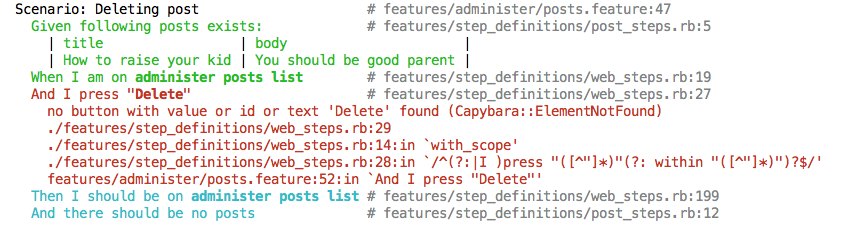
\includegraphics[width=\linewidth]{images/scenario_failure_2.png}
   			\caption{Nowo dodany scenariusz nie przechodzi, wszystkie kroki są zdefiniowane.}
   			\label{scenario_failure_2}
   		\end{center}
   	\end{figure}
  
  \section{Wnioski}
